\subsection{Radix Sort}

\subsubsection{Core Concepts}
Radix sort is an algorithm that does not use comparisons to sorted the array. To be specific, treats each data item as a character string, groups the data items according to the rightmost character then put these groups into order with respect to this rightmost character, combine all the groups and move to the next left position. At the end, the sort operation will be in sorted. ~\cite{ref1}

\vspace{3pt}

\subsubsection{Step-by-step Explaination}
\begin{itemize}[label=-]
    \item Step 1: find max value by calling getMax to determine the maximum number in the array.
    \item Step 2: Start with the rightmost significant number. Apply countSort to sort the array based on the current number. Move to the next significant digit by multiplying exp by 10. Repeat the process until all digits have been processed (when m / exp becomes 0).
\end{itemize}

\subsubsection{Complexity Analysis}
\textbf{Time Complexity: }
\begin{itemize}
    \item Radix sort is a non-comparative integer sorting algorithm that sorts data with integer keys by grouping the keys by the individual digits which share the same significant position and value. It has a time complexity of $O(d \cdot (n + b))$, where d is the number of digits, n is the number of elements, and b is the base of the number system being used.
    \item In practical implementations, radix sort is often faster than other comparison-based sorting algorithms, such as quicksort or merge sort, for large datasets, especially when the keys have many digits. However, its time complexity grows linearly with the number of digits, and so it is not as efficient for small datasets. ~\cite{ref5}
\end{itemize}

\textbf{Space complexity: }
Radix sort also has a space complexity of $O(n + b)$, where n is the number of elements and b is the base of the number system. This space complexity comes from the need to create buckets for each digit value and to copy the elements back to the original array after each digit has been sorted.

\textbf{An example of radix sort:} ~\cite{ref2}

\begin{figure}[h]
    \centering
    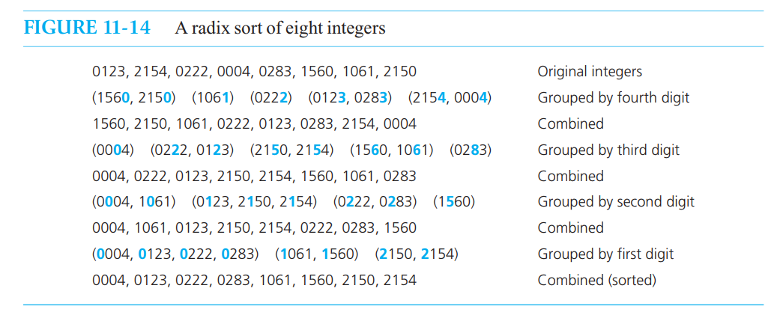
\includegraphics[width=1.\textwidth]{Figures/sort_demo/radix.png}
    \caption{Radix Sort Demo}
    \label{fig:enter-label}
\end{figure}